% Options for packages loaded elsewhere
\PassOptionsToPackage{unicode}{hyperref}
\PassOptionsToPackage{hyphens}{url}
%
\documentclass[
  english,
  man]{apa6}
\usepackage{lmodern}
\usepackage{amssymb,amsmath}
\usepackage{ifxetex,ifluatex}
\ifnum 0\ifxetex 1\fi\ifluatex 1\fi=0 % if pdftex
  \usepackage[T1]{fontenc}
  \usepackage[utf8]{inputenc}
  \usepackage{textcomp} % provide euro and other symbols
\else % if luatex or xetex
  \usepackage{unicode-math}
  \defaultfontfeatures{Scale=MatchLowercase}
  \defaultfontfeatures[\rmfamily]{Ligatures=TeX,Scale=1}
\fi
% Use upquote if available, for straight quotes in verbatim environments
\IfFileExists{upquote.sty}{\usepackage{upquote}}{}
\IfFileExists{microtype.sty}{% use microtype if available
  \usepackage[]{microtype}
  \UseMicrotypeSet[protrusion]{basicmath} % disable protrusion for tt fonts
}{}
\makeatletter
\@ifundefined{KOMAClassName}{% if non-KOMA class
  \IfFileExists{parskip.sty}{%
    \usepackage{parskip}
  }{% else
    \setlength{\parindent}{0pt}
    \setlength{\parskip}{6pt plus 2pt minus 1pt}}
}{% if KOMA class
  \KOMAoptions{parskip=half}}
\makeatother
\usepackage{xcolor}
\IfFileExists{xurl.sty}{\usepackage{xurl}}{} % add URL line breaks if available
\IfFileExists{bookmark.sty}{\usepackage{bookmark}}{\usepackage{hyperref}}
\hypersetup{
  pdftitle={TV Consumption and Government Approval in Russia},
  pdfauthor={Evgeniya Mitrokhina1},
  pdflang={en-EN},
  pdfkeywords={media persuasion, public opinion, authoritarian regimes},
  hidelinks,
  pdfcreator={LaTeX via pandoc}}
\urlstyle{same} % disable monospaced font for URLs
\usepackage{longtable,booktabs}
% Correct order of tables after \paragraph or \subparagraph
\usepackage{etoolbox}
\makeatletter
\patchcmd\longtable{\par}{\if@noskipsec\mbox{}\fi\par}{}{}
\makeatother
% Allow footnotes in longtable head/foot
\IfFileExists{footnotehyper.sty}{\usepackage{footnotehyper}}{\usepackage{footnote}}
\makesavenoteenv{longtable}
\usepackage{graphicx,grffile}
\makeatletter
\def\maxwidth{\ifdim\Gin@nat@width>\linewidth\linewidth\else\Gin@nat@width\fi}
\def\maxheight{\ifdim\Gin@nat@height>\textheight\textheight\else\Gin@nat@height\fi}
\makeatother
% Scale images if necessary, so that they will not overflow the page
% margins by default, and it is still possible to overwrite the defaults
% using explicit options in \includegraphics[width, height, ...]{}
\setkeys{Gin}{width=\maxwidth,height=\maxheight,keepaspectratio}
% Set default figure placement to htbp
\makeatletter
\def\fps@figure{htbp}
\makeatother
\setlength{\emergencystretch}{3em} % prevent overfull lines
\providecommand{\tightlist}{%
  \setlength{\itemsep}{0pt}\setlength{\parskip}{0pt}}
\setcounter{secnumdepth}{-\maxdimen} % remove section numbering
% Make \paragraph and \subparagraph free-standing
\ifx\paragraph\undefined\else
  \let\oldparagraph\paragraph
  \renewcommand{\paragraph}[1]{\oldparagraph{#1}\mbox{}}
\fi
\ifx\subparagraph\undefined\else
  \let\oldsubparagraph\subparagraph
  \renewcommand{\subparagraph}[1]{\oldsubparagraph{#1}\mbox{}}
\fi
% Manuscript styling
\usepackage{upgreek}
\captionsetup{font=singlespacing,justification=justified}

% Table formatting
\usepackage{longtable}
\usepackage{lscape}
% \usepackage[counterclockwise]{rotating}   % Landscape page setup for large tables
\usepackage{multirow}		% Table styling
\usepackage{tabularx}		% Control Column width
\usepackage[flushleft]{threeparttable}	% Allows for three part tables with a specified notes section
\usepackage{threeparttablex}            % Lets threeparttable work with longtable

% Create new environments so endfloat can handle them
% \newenvironment{ltable}
%   {\begin{landscape}\begin{center}\begin{threeparttable}}
%   {\end{threeparttable}\end{center}\end{landscape}}
\newenvironment{lltable}{\begin{landscape}\begin{center}\begin{ThreePartTable}}{\end{ThreePartTable}\end{center}\end{landscape}}

% Enables adjusting longtable caption width to table width
% Solution found at http://golatex.de/longtable-mit-caption-so-breit-wie-die-tabelle-t15767.html
\makeatletter
\newcommand\LastLTentrywidth{1em}
\newlength\longtablewidth
\setlength{\longtablewidth}{1in}
\newcommand{\getlongtablewidth}{\begingroup \ifcsname LT@\roman{LT@tables}\endcsname \global\longtablewidth=0pt \renewcommand{\LT@entry}[2]{\global\advance\longtablewidth by ##2\relax\gdef\LastLTentrywidth{##2}}\@nameuse{LT@\roman{LT@tables}} \fi \endgroup}

% \setlength{\parindent}{0.5in}
% \setlength{\parskip}{0pt plus 0pt minus 0pt}

% \usepackage{etoolbox}
\makeatletter
\patchcmd{\HyOrg@maketitle}
  {\section{\normalfont\normalsize\abstractname}}
  {\section*{\normalfont\normalsize\abstractname}}
  {}{\typeout{Failed to patch abstract.}}
\patchcmd{\HyOrg@maketitle}
  {\section{\protect\normalfont{\@title}}}
  {\section*{\protect\normalfont{\@title}}}
  {}{\typeout{Failed to patch title.}}
\makeatother
\shorttitle{TV Consumption and Government Approval in Russia}
\keywords{media persuasion, public opinion, authoritarian regimes\newline\indent Word count: X}
\DeclareDelayedFloatFlavor{ThreePartTable}{table}
\DeclareDelayedFloatFlavor{lltable}{table}
\DeclareDelayedFloatFlavor*{longtable}{table}
\makeatletter
\renewcommand{\efloat@iwrite}[1]{\immediate\expandafter\protected@write\csname efloat@post#1\endcsname{}}
\makeatother
\usepackage{lineno}

\linenumbers
\usepackage{csquotes}
\ifxetex
  % Load polyglossia as late as possible: uses bidi with RTL langages (e.g. Hebrew, Arabic)
  \usepackage{polyglossia}
  \setmainlanguage[]{english}
\else
  \usepackage[shorthands=off,main=english]{babel}
\fi

\title{TV Consumption and Government Approval in Russia}
\author{Evgeniya Mitrokhina\textsuperscript{1}}
\date{}


\authornote{

PhD student at UW-Madison

}

\affiliation{\vspace{0.5cm}\textsuperscript{1} UW-Madison}

\abstract{
During the last four years Russia is suffering from the economic crisis caused by the Crimea annexation and sanctions induced by foreign countries. At the same time, pro-government media provide such content that emphasizes mostly positive consequences of these events, whereas the economic well-being of Russian citizens has deteriorated. In the work I try to understand whether TV consumption affects government approval. To do so I analyse public opinion data collected from July 2018 to October 2019. I find the possitive correlation between the frequency of TV consumption and the approval of the President and governors. However, people who use the Internet tend to disapprve the government.
}



\begin{document}
\maketitle

\hypertarget{introduction}{%
\section{Introduction}\label{introduction}}

Many scholars highlight that modern autocrats differ from the classical understanding of dictatorship. The strategies autocrats use to hold on to the power are also changing. It relates to the developing technologies and its introduction to a daily life of people as well as tools, that governments use to control them. Modern authoritarian regimes more frequently use media to persuade citizens and legitimate their rule. With much less violence and fear, authorities in these countries seek to convince citizens in the governments' competence. That is why in the work I would like to investigate the association between officials approval and frequency of watching the TV.

Authoritarian regimes develop new techniques to prolong their existence. Scholars argue that modern autocrats pay more attention to information and its effect on public opinion (Guriev \& Treisman, 2018, 2020; Roberts, 2018; Sanovich, Stukal, \& Tucker, 2018; Tucker et al., 2018). The use of and control over the media is an essential tool. The manipulation of the information by autocrats implies that public is less aware of the censorship than the elite, and as a result the informational autocrats should be more popular with the public than the elite. Autocrats today tend to mimic democratic rulers not only establishing institutions but using the same communication with citizens and emphasizing economic performance and public provisions.

Autocrats cannot solely rely on repression, they need some additional tools to be able to accumulate more power, in these circumstances loyalty of citizens is instrumental to the survival of a dictatorships. To keep the power leaders must discourage their ruling coalition and outside rivals to subvert their rule. One of the ways to do it is to convince them in that is to create an image of invincibility (Magaloni \& Wallace, 2008). Manufacturing this image allows dictators to signal opponents that attempts to rebel are pointless because the leader is indestructible. The image is assuring the public that the leader is popular and supported by many that cause less disobedience even if some citizens are aggrieved. Thus, the popularity of the regime and its strength becomes a common knowledge.

Various studies examined how media affect political participation, news consumption and its effect on electoral outcomes in democracies (Gentzkow, Shapiro, \& Sinkinson, 2011; Petrova, 2011) as well as in not liberal regimes (Adena, Enikolopov, Petrova, Santarosa, \& Zhuravskaya, 2015; Enikolopov, Petrova, \& Zhuravskaya, 2011; Knight \& Tribin, 2019; Larreguy \& Marshall, 2019). Studies of media control and propaganda in authoritarian regimes have implications for literature about the regime endurance (Chen \& Xu, 2015; King, Pan, \& Roberts, 2014; Lankina \& Watanabe, 2017). Media censorship is effective as a mechanism to constrain expression of antigovernment sentiment.At the same time, however, it is costly to maintain and implement (King, Pan, \& Roberts, 2013). Independent media in autocracies may lead to erosion of a regime's legitimacy and even challenge the stability of authoritarian rule (Egorov, Guriev, \& Sonin, 2009; Enikolopov et al., 2011; Levitsky \& Way, 2002). Therefore, autocrats have incentives to limit the activities of media outlets that do not support the government.

Comparative studies present evidence that people in democratic countries on average have higher levels of trust in media (Tsfati \& Ariely, 2014). Thus, people in authoritarian regimes should be more skeptical about the media, especially about the state-affiliated outlets (Wedeen, 2015). Some citizens discount the information that receive from state-owned media outlets because of inconsistencies with their own experience and other information sources (Mickiewicz, 2008). However, according to Levada surveys, Russians find television trustworthy although it is controlled by the government. That is why it is possible to assume that the bias translated through the media is not necessarily an obstacle for its consumers, and as a result it affects their views. At the same time, those who do not trust television more willingly consume the Internet.

In the work I try to understand whether TV consumption affects government approval. Based on the literature I highlight several hypotheses:

\begin{enumerate}
\def\labelenumi{\arabic{enumi}.}
\item
  Frequency of watching TV has different effect on the approval of political actors (the level of power)
\item
  People who watch state-owned TV channels are more likely to approve Russian officials policy
\item
  People who use the Internet are more likely to disapprove Russian officials policy
\end{enumerate}

\hypertarget{data-and-methods}{%
\section{Data and methods}\label{data-and-methods}}

For the project I use survey data. The survey was conducted by \href{https://bd.wciom.ru/baza_dannykh_roper_center/}{VCIOM} (a Russian polling agency) from July \(2018\) to October \(2019\). The survey is representative on the country level conducted in \(80\) Russian regions every day (\(\approx 48000\) respondents each month). As the \textbf{dependent variable} I use approval of the President and the Governor (head of a region, republic). As the main \textbf{independent variable} I use frequency of watching TV (where \(1\) denotes not TV at all, and \(6\) denotes watching TV every day more than \(4\) hours per day). I would also test the hypothesis about the association if using the Internet and officials approval (the variable for the frequncy of using the internet is coded the same as the one for TV). I also use a set of \textbf{control variables}, they are socio-economic variables (gender, education, income). The summary statistics are shown in the table 1. Because I have time-varying data I am able to trace the changes in approval ratings, they are shown on the figure 1.

Because I have a binary dependent variable, I am using logistic regression testing the model for the President and the Governor. Using the method is appropriate for binary outcomes, input variables that have any measurement level, and predicted values are the probability of a particular level(s) of target variable at the given values of input variables.

\begin{longtable}[]{@{}lrrrr@{}}
\caption{\label{tab:unnamed-chunk-2}Summary statistics}\tabularnewline
\toprule
& Mean & SD & Min & Max\tabularnewline
\midrule
\endfirsthead
\toprule
& Mean & SD & Min & Max\tabularnewline
\midrule
\endhead
\enquote{President approval} & 0.70 & 0.46 & 0.00 & 1.00\tabularnewline
\enquote{Governor approval} & 0.70 & 0.46 & 0.00 & 1.00\tabularnewline
\enquote{TV watching frequncy} & 4.46 & 1.48 & 1.00 & 6.00\tabularnewline
\enquote{Internet frequncy} & 4.28 & 1.78 & 1.00 & 6.00\tabularnewline
\bottomrule
\end{longtable}

\begin{figure}[h]
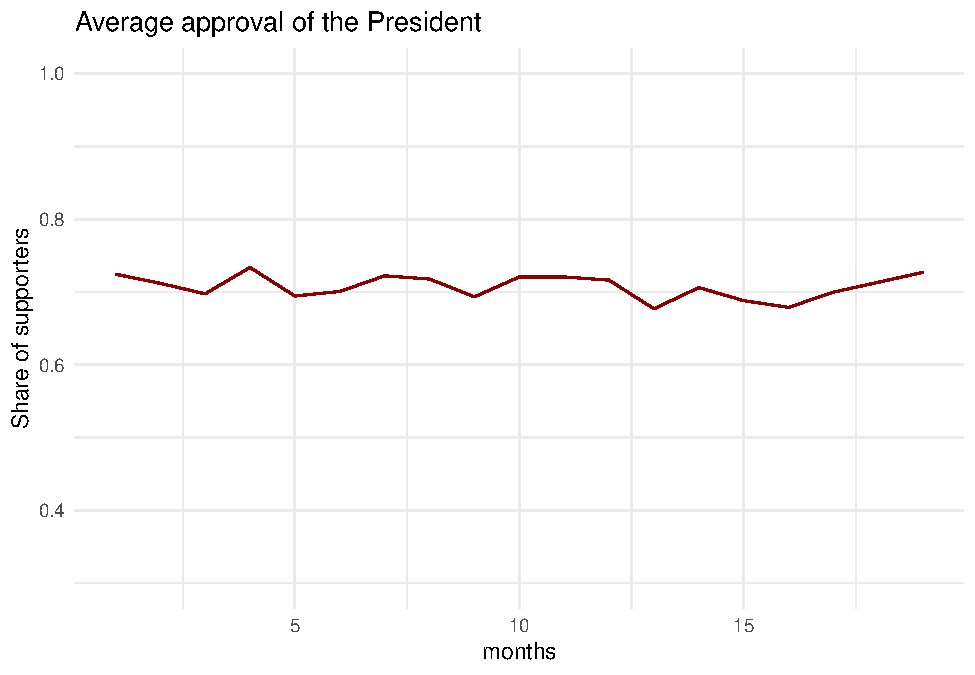
\includegraphics[width=0.5\linewidth,]{Final_paper_files/figure-latex/figures-side-1} 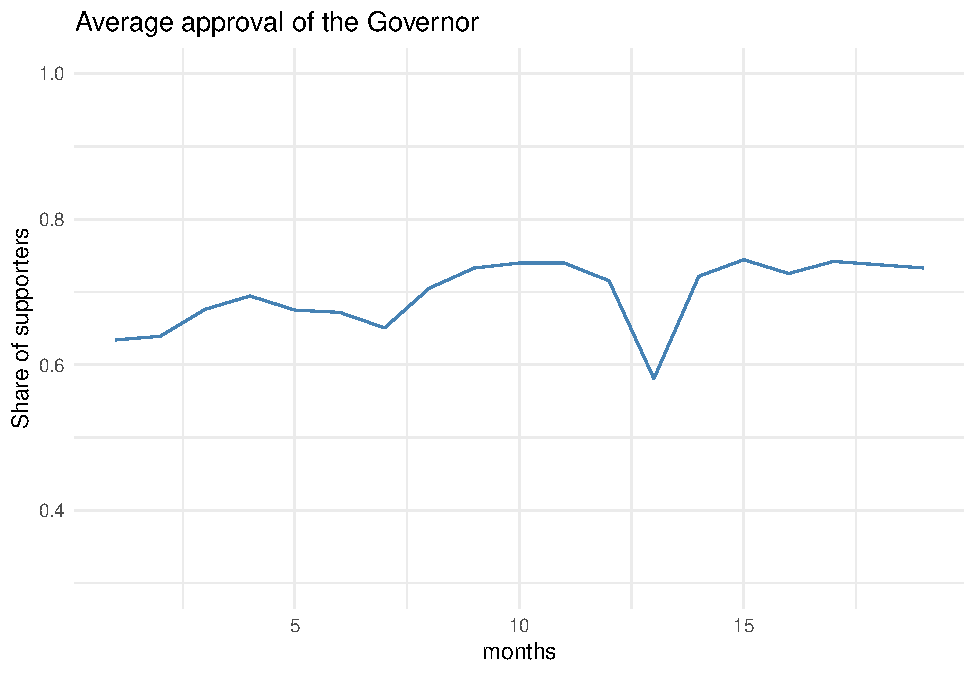
\includegraphics[width=0.5\linewidth,]{Final_paper_files/figure-latex/figures-side-2} \caption{ }\label{fig:figures-side}
\end{figure}

\hypertarget{results}{%
\section{Results}\label{results}}

\begin{table}[!htbp] \centering 
  \caption{Political actors approval assosiated with watching TV frequency} 
  \label{} 
\small 
\begin{tabular}{@{\extracolsep{5pt}}lcc} 
\\[-1.8ex]\hline 
\hline \\[-1.8ex] 
 & \multicolumn{2}{c}{\textit{Dependent variable:}} \\ 
\cline{2-3} 
\\[-1.8ex] & President approval & Governor approval \\ 
\\[-1.8ex] & (1) & (2)\\ 
\hline \\[-1.8ex] 
 TV very rarely & 0.029 & $-$0.032 \\ 
  & (0.212) & (0.215) \\ 
  & & \\ 
 Several times per month & 0.446$^{**}$ & 0.111 \\ 
  & (0.185) & (0.188) \\ 
  & & \\ 
 Several times per week & 0.636$^{***}$ & 0.304$^{**}$ \\ 
  & (0.146) & (0.149) \\ 
  & & \\ 
 Every day less than 4hrs & 0.886$^{***}$ & 0.395$^{***}$ \\ 
  & (0.143) & (0.143) \\ 
  & & \\ 
 Every day more than 4hrs & 1.092$^{***}$ & 0.537$^{***}$ \\ 
  & (0.178) & (0.172) \\ 
  & & \\ 
 Age & 0.504 & 17.524 \\ 
  & (1.369) & (956.867) \\ 
  & & \\ 
\hline \\[-1.8ex] 
Observations & 2,816 & 2,816 \\ 
Log Likelihood & $-$1,471.766 & $-$1,523.380 \\ 
Akaike Inf. Crit. & 3,177.532 & 3,280.759 \\ 
\hline 
\hline \\[-1.8ex] 
\textit{Note:}  & \multicolumn{2}{r}{$^{*}$p$<$0.1; $^{**}$p$<$0.05; $^{***}$p$<$0.01} \\ 
\end{tabular} 
\end{table}

\begin{table}[!htbp] \centering 
  \caption{Political actors approval assosiated with using the Internet} 
  \label{} 
\small 
\begin{tabular}{@{\extracolsep{5pt}}lcc} 
\\[-1.8ex]\hline 
\hline \\[-1.8ex] 
 & \multicolumn{2}{c}{\textit{Dependent variable:}} \\ 
\cline{2-3} 
\\[-1.8ex] & President approval & Governor approval \\ 
\\[-1.8ex] & (1) & (2)\\ 
\hline \\[-1.8ex] 
 Very rarely & $-$0.930$^{**}$ & 0.006 \\ 
  & (0.407) & (0.417) \\ 
  & & \\ 
 Several times per month & $-$0.913$^{**}$ & $-$0.268 \\ 
  & (0.414) & (0.401) \\ 
  & & \\ 
 Several times per week & $-$0.839$^{***}$ & $-$0.893$^{***}$ \\ 
  & (0.258) & (0.222) \\ 
  & & \\ 
 Every day less than 4hrs & $-$1.331$^{***}$ & $-$0.931$^{***}$ \\ 
  & (0.222) & (0.193) \\ 
  & & \\ 
 Every day more than 4hrs & $-$1.397$^{***}$ & $-$1.086$^{***}$ \\ 
  & (0.235) & (0.208) \\ 
  & & \\ 
 Age & 0.504 & 17.524 \\ 
  & (1.369) & (956.867) \\ 
  & & \\ 
\hline \\[-1.8ex] 
Observations & 2,816 & 2,816 \\ 
Log Likelihood & $-$1,471.766 & $-$1,523.380 \\ 
Akaike Inf. Crit. & 3,177.532 & 3,280.759 \\ 
\hline 
\hline \\[-1.8ex] 
\textit{Note:}  & \multicolumn{2}{r}{$^{*}$p$<$0.1; $^{**}$p$<$0.05; $^{***}$p$<$0.01} \\ 
\end{tabular} 
\end{table}

\hypertarget{discussion}{%
\section{Discussion}\label{discussion}}

\newpage

\hypertarget{references}{%
\section{References}\label{references}}

\begingroup
\setlength{\parindent}{-0.5in}
\setlength{\leftskip}{0.5in}

\hypertarget{refs}{}
\leavevmode\hypertarget{ref-adenaRadioRiseNazis2015}{}%
Adena, M., Enikolopov, R., Petrova, M., Santarosa, V., \& Zhuravskaya, E. (2015). Radio and the Rise of the Nazis in Prewar Germany. \emph{The Quarterly Journal of Economics}, \emph{130}(4), 1885--1939.

\leavevmode\hypertarget{ref-chenInformationManipulationReform2015}{}%
Chen, J., \& Xu, Y. (2015). Information manipulation and reform in authoritarian regimes. \emph{Forthcoming in Political Science Research and Methods}, 2014--2021.

\leavevmode\hypertarget{ref-egorovWhyResourcepoorDictators2009}{}%
Egorov, G., Guriev, S., \& Sonin, K. (2009). Why resource-poor dictators allow freer media: A theory and evidence from panel data. \emph{American Political Science Review}, 645--668.

\leavevmode\hypertarget{ref-enikolopovMediaPoliticalPersuasion2011}{}%
Enikolopov, R., Petrova, M., \& Zhuravskaya, E. (2011). Media and political persuasion: Evidence from Russia. \emph{American Economic Review}, \emph{101}(7), 3253--3285.

\leavevmode\hypertarget{ref-gentzkowEffectNewspaperEntry2011}{}%
Gentzkow, M., Shapiro, J. M., \& Sinkinson, M. (2011). The effect of newspaper entry and exit on electoral politics. \emph{American Economic Review}, \emph{101}(7), 2980--3018.

\leavevmode\hypertarget{ref-gurievInformationalAutocracyTheory2018}{}%
Guriev, S., \& Treisman, D. (2018). Informational Autocracy: Theory and Empirics of Modern Authoritarianism. \emph{Available at SSRN 2571905}.

\leavevmode\hypertarget{ref-gurievTheoryInformationalAutocracy2020}{}%
Guriev, S., \& Treisman, D. (2020). A theory of informational autocracy. \emph{Journal of Public Economics}, \emph{186}, 104158.

\leavevmode\hypertarget{ref-kingHowCensorshipChina2013}{}%
King, G., Pan, J., \& Roberts, M. E. (2013). How censorship in China allows government criticism but silences collective expression. \emph{American Political Science Review}, 326--343.

\leavevmode\hypertarget{ref-kingReverseengineeringCensorshipChina2014}{}%
King, G., Pan, J., \& Roberts, M. E. (2014). Reverse-engineering censorship in China: Randomized experimentation and participant observation. \emph{Science}, \emph{345}(6199).

\leavevmode\hypertarget{ref-knightLimitsPropagandaEvidence2019}{}%
Knight, B., \& Tribin, A. (2019). The limits of propaganda: Evidence from chavez's venezuela. \emph{Journal of the European Economic Association}, \emph{17}(2), 567--605.

\leavevmode\hypertarget{ref-lankinaRussianSpringSpring2017}{}%
Lankina, T., \& Watanabe, K. (2017). `Russian Spring'or ``Spring betrayal''? The media as a mirror of Putin's evolving strategy in Ukraine. \emph{Europe-Asia Studies}, \emph{69}(10), 1526--1556.

\leavevmode\hypertarget{ref-larreguyIncentivesEffectsIndependent2019}{}%
Larreguy, H., \& Marshall, J. (2019). The incentives and effects of independent and government-controlled media in the developing world. In \emph{The Oxford Handbook of Electoral Persuasion}.

\leavevmode\hypertarget{ref-levitskyElectionsDemocracyRise2002}{}%
Levitsky, S., \& Way, L. A. (2002). Elections without democracy: The rise of competitive authoritarianism. \emph{Journal of Democracy}, \emph{13}(2), 51--65.

\leavevmode\hypertarget{ref-magaloniCitizenLoyaltyMass2008}{}%
Magaloni, B., \& Wallace, J. (2008). Citizen loyalty, mass protest and authoritarian survival. In \emph{Conference on dictatorships: Their governance and social consequences, princeton university}.

\leavevmode\hypertarget{ref-mickiewiczTelevisionPowerPublic2008}{}%
Mickiewicz, E. P. (2008). \emph{Television, power, and the public in Russia}. Cambridge university press,

\leavevmode\hypertarget{ref-petrovaNewspapersPartiesHow2011}{}%
Petrova, M. (2011). Newspapers and parties: How advertising revenues created an independent press. \emph{American Political Science Review}, 790--808.

\leavevmode\hypertarget{ref-robertsCensoredDistractionDiversion2018}{}%
Roberts, M. E. (2018). \emph{Censored: Distraction and diversion inside China's Great Firewall}. Princeton University Press.

\leavevmode\hypertarget{ref-sanovichTurningVirtualTables2018}{}%
Sanovich, S., Stukal, D., \& Tucker, J. A. (2018). Turning the virtual tables: Government strategies for addressing online opposition with an application to Russia. \emph{Comparative Politics}, \emph{50}(3), 435--482.

\leavevmode\hypertarget{ref-tsfatiIndividualContextualCorrelates2014}{}%
Tsfati, Y., \& Ariely, G. (2014). Individual and contextual correlates of trust in media across 44 countries. \emph{Communication Research}, \emph{41}(6), 760--782.

\leavevmode\hypertarget{ref-tuckerSocialMediaPolitical2018}{}%
Tucker, J. A., Guess, A., Barberá, P., Vaccari, C., Siegel, A., Sanovich, S., \ldots{} Nyhan, B. (2018). Social media, political polarization, and political disinformation: A review of the scientific literature. \emph{Political Polarization, and Political Disinformation: A Review of the Scientific Literature (March 19, 2018)}.

\leavevmode\hypertarget{ref-wedeenAmbiguitiesDominationPolitics2015}{}%
Wedeen, L. (2015). \emph{Ambiguities of domination: Politics, rhetoric, and symbols in contemporary Syria}. University of Chicago Press.

\endgroup


\end{document}
